\documentclass[final]{beamer}
\usepackage[orientation=portrait,size=a1,scale=1.2,debug]{beamerposter}
%\usepackage[size=custom,width=24.75in,height=35in,scale=2,debug]{beamerposter}

\mode<presentation>{\usetheme{CoEPPoster}}
\usepackage[english]{babel}
%\usepackage[latin1]{inputenc}
\usepackage[T1]{fontenc}
\usepackage{amsmath,amsthm, amssymb, latexsym}

\usepackage[disable]{todonotes} % To remove in-line review comments, use 'disable'
%\usepackage[colorinlistoftodos,textsize=normalsize,textwidth=1\marginparwidth]{todonotes} % To add in-line review comments

\usepackage{array,booktabs,tabularx}
\newcolumntype{Z}{>{\centering\arraybackslash}X} % centered tabularx columns

% comment 
\newcommand{\comment}[1]{}

% (relative) path to the figures
%\graphicspath{{../Common/images/}}
\newcommand{\generic}[7]{\ensuremath{#1{\bf \mathcal{#2}}_{#3}^{#4,#5} [\{#6\} (#7)]}}

\newlength{\columnheight}
\setlength{\columnheight}{105cm}
\newlength{\sepwid}
\newlength{\onecolwid}
\newlength{\twocolwid}
\newlength{\threecolwid}
\setlength{\sepwid}{0.024\paperwidth}
\setlength{\onecolwid}{0.24\paperwidth}
\setlength{\twocolwid}{0.4\paperwidth}
\setlength{\threecolwid}{0.19\paperwidth}

\author{Yogesh H Kulkarni, Anil Sahasrabudhe, Mukund Kale}
\institute[CoEP]{College of Engineering Pune}
\subtitle[]{Development of algorithms for generating connected midsurfaces using feature information in thin-walled parts}

\usepackage[disable]{todonotes} % To remove in-line review comments, use 'disable'
%\usepackage[colorinlistoftodos,textsize=normalsize,textwidth=1\marginparwidth]{todonotes} % To add in-line review comments

% ---------------------------------------------------------------------------------------------------% 
% Title, author, date, etc.
% ---------------------------------------------------------------------------------------------------% 
\title{\huge Abstracting Thin-walled Solids to Surfaces}

\date[]{}
%%% Put the name of conference here.
	%\def\conference{Autodesk University India \& SAARC 2014} 
	\def\conference{}
 %%% Put your e-mail address here.
 	\def\yourEmail{kulkarniyh12.mech@coep.ac.in}


% ---------------------------------------------------------------------------------------------------% 
% Contents
% ---------------------------------------------------------------------------------------------------% 
\begin{document}
\begin{frame}[t]
\begin{columns}[t]

% -----------------------------------------------------------
% Start the first column
% -----------------------------------------------------------
\begin{column}{\twocolwid}


% -----------------------------------------------------------
\begin{block}{Why reduce dimension?}
\baselineskip=.7\baselineskip
\begin{itemize}
\item For quick CAE analysis of Thin-walled parts
\begin{itemize}
\item 3D meshing is expensive wrt time-resources
\item Need min 3 levels of elements along thickness;
\end{itemize}
\item Also, to find Principal shape, useful in
\begin{itemize}
\item Shape matching, Retrieval
\item Data transmission, Level of Details
\end{itemize}
\end{itemize}
\bigskip
\textbf{Midsurface} represents idealized thin-walled solid
\end{block}
% -----------------------------------------------------------


\begin{block}{How to reduce dimension?}
\begin{center}
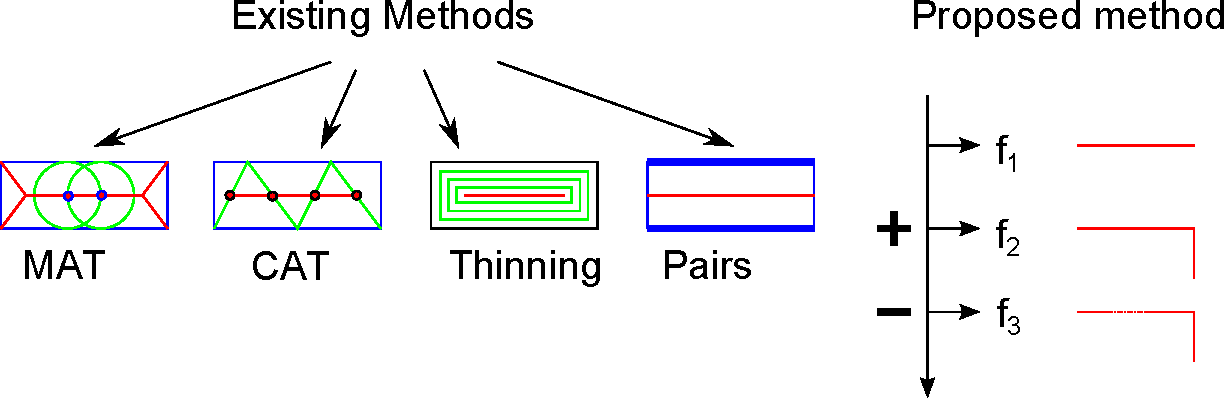
\includegraphics[width=0.9\linewidth]{../Common/images/MedialMethods.pdf}
\end{center}
\end{block}

\begin{block}{Whats the problem?}
\begin{center}
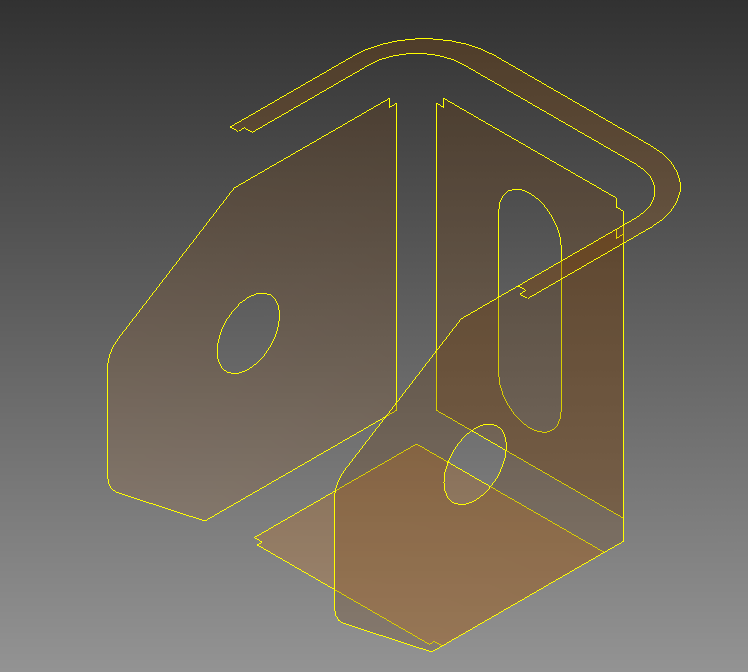
\includegraphics[scale=0.6]{../Common/images/Inventor_Bracket_MidsBorders.png}
\end{center}
Need the \textbf{Midsurface} to mimic the original shape continuously, with no gaps, overlaps
\end{block}

\begin{block}{Workflow}
\begin{center}
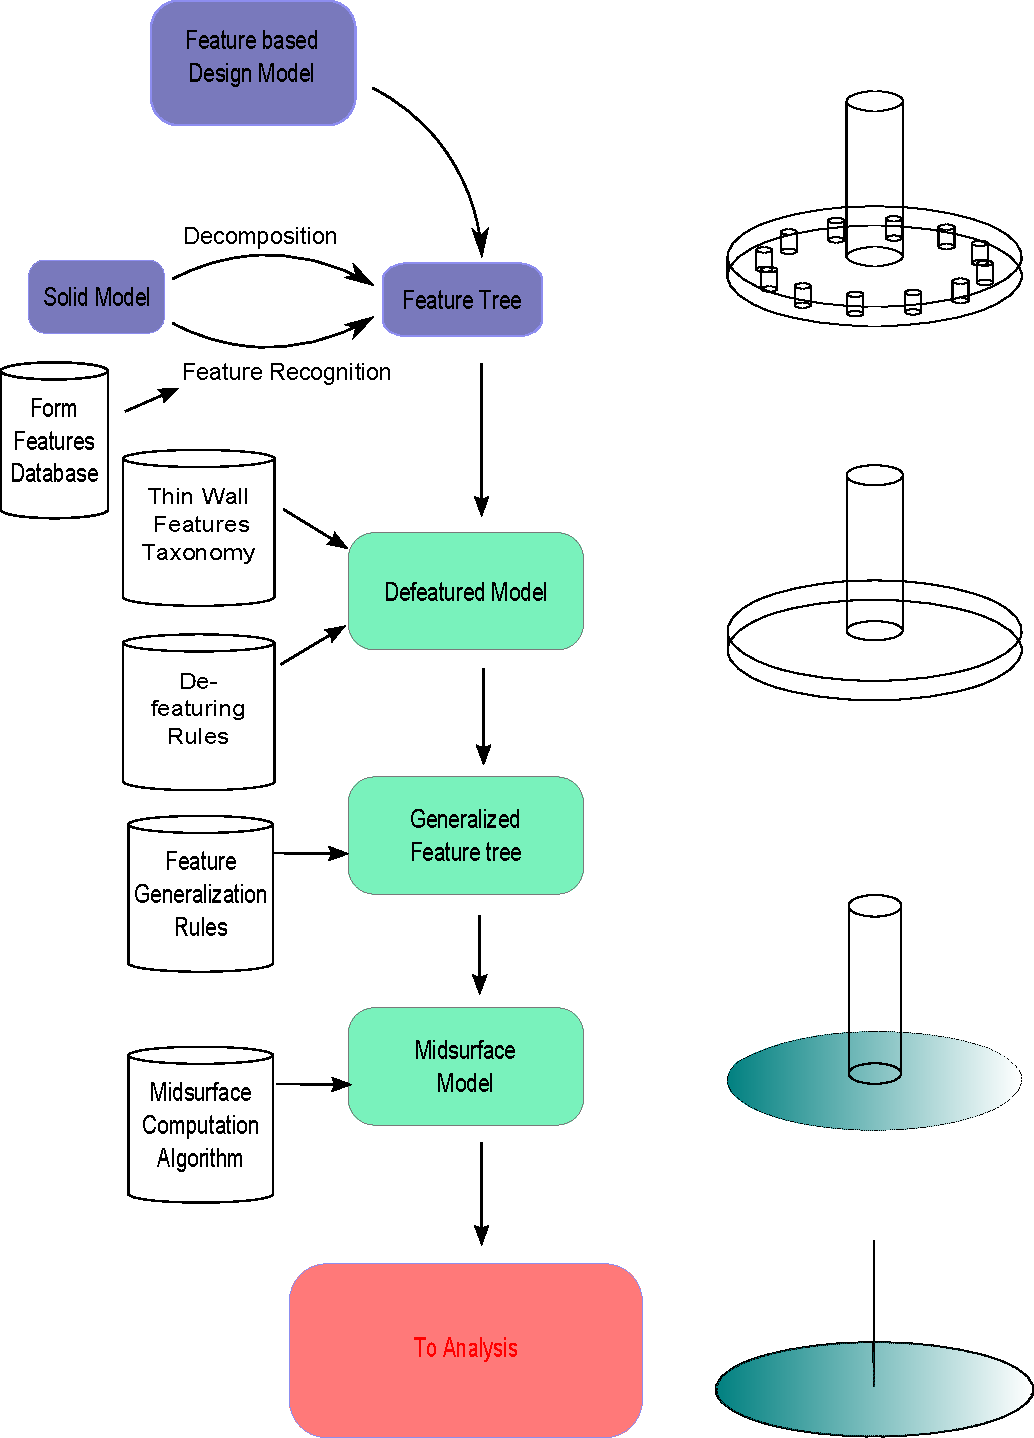
\includegraphics[width=0.6\linewidth]{../Common/images/SystemArchitecture.pdf}
\end{center}
\end{block}
\end{column}

% -----------------------------------------------------------
% Start the second column
% -----------------------------------------------------------
\begin{column}{\twocolwid}
% -----------------------------------------------------------

\begin{block}{What's the approach?}
\textbf{Divide and Conquer}
\begin{itemize}
\item Divide the shape into sub-shapes
\item Find Midsurface for individual sub-shapes
\item Connect individual Midsurfaces at the interfaces
\end{itemize}
\end{block}

\begin{block}{How to get sub-shapes?}

\begin{tabular}{@{}p{0.45\linewidth}p{0.4\linewidth}@{}}
\begin{itemize}
\item \textbf{2D-Profile}: Polygon Decomposition
\item \textbf{3D-Shapes, 1st level}: Feature-tree
\item \textbf{3D-Shapes, 2nd level}: Remnant Faces, Cellular Decomposition
\end{itemize} 
&
\raisebox{-0.9\height}{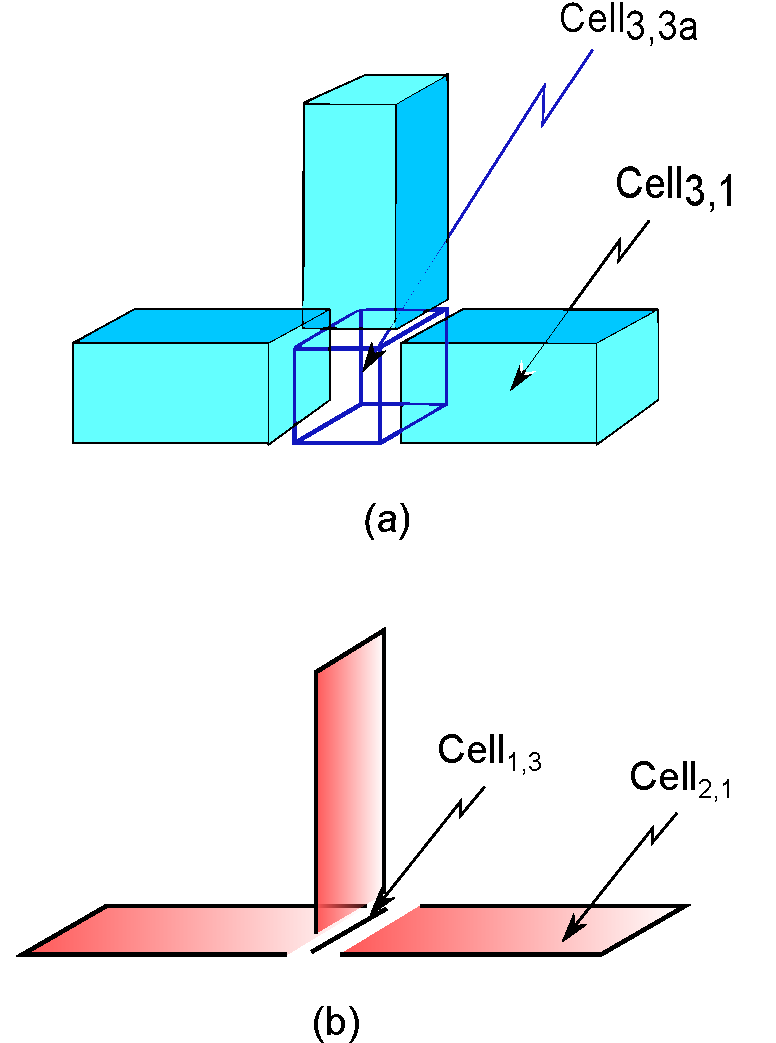
\includegraphics[scale=0.6]{../Common/images/Cellular_Topology.pdf}}\\
\end{tabular}

\end{block}


\begin{block}{Abstracting features}

\begin{tabular}{@{}p{0.45\linewidth}p{0.4\linewidth}@{}}
Loft is a generic operator capable of generating most of the basic shapes. It joins {\em profiles} along a guide {\em curve}. 
Represented as:

\ensuremath{\textcolor{magenta}{\Omega{\bf \mathcal{L}}_{}^{subtype,3}}[\textcolor{blue}{\{0, curve, 0 | C_{0,1,2}\}}\textcolor{red}{( (sketch )^{<1-n>})}]}

%\loft{}{subtype}{3}{0, curve, 0 | C_{0,1,2}}{ (sketch )^{<1-n>}}
&
\raisebox{-0.9\height}{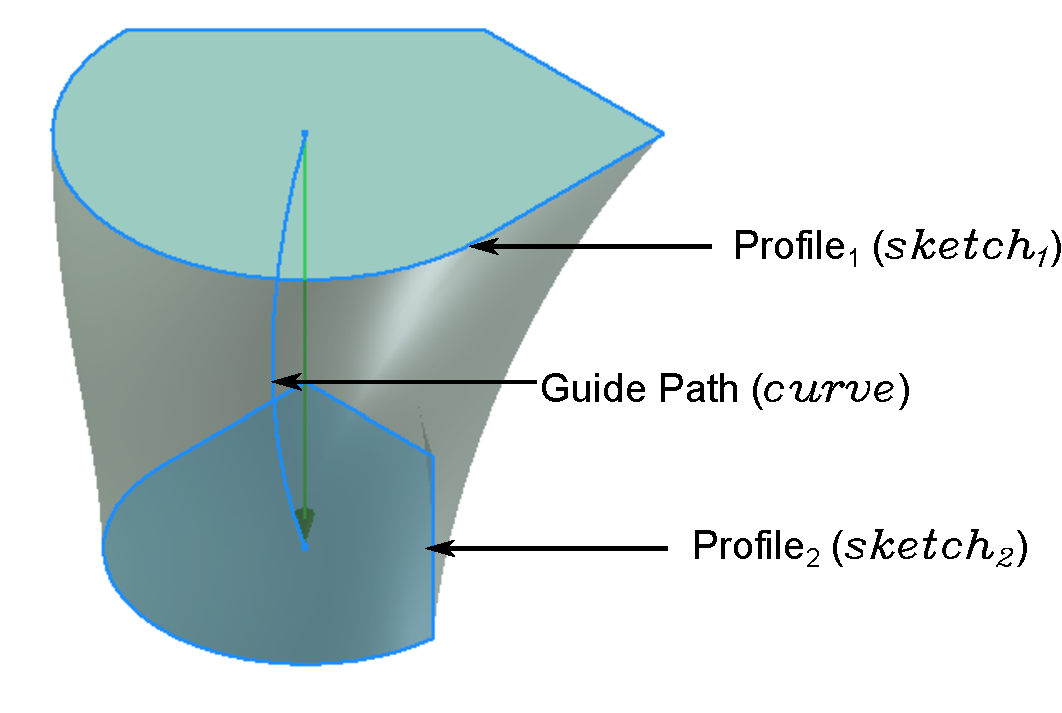
\includegraphics[scale=0.6]{../Common/images/LoftPreview.pdf}}\\

\end{tabular}

\end{block}


\begin{block}{Midsurface}

To generate Midsurface of a Swept volume, Midcurves of the profile are calculated first and then swept similar to that of parent volume.

\vspace{1cm}
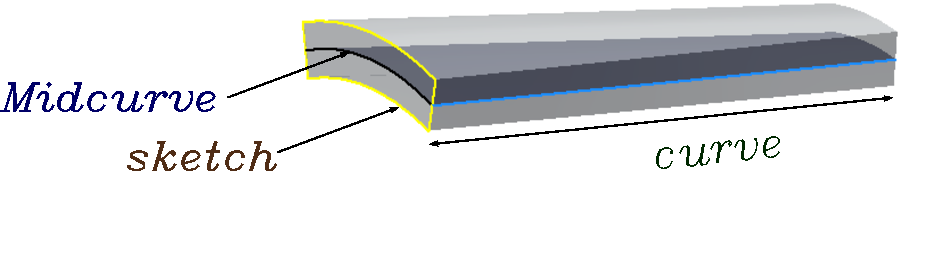
\includegraphics[width=0.9\linewidth]{../Common/images/MidsurfSmallProfile.pdf}

\ensuremath{\textcolor{magenta}{\Omega{\bf \mathcal{L}}_{}^{subtype,2}}[\textcolor{blue}{\{0, curve, 0 | C_{0,1,2}\}}\textcolor{red}{( midcurve^{1-n})}]}
%\loft{}{L}{2}{0, curve, 0 | C_{0,1,2}}{midcurve^{1-n}} 
\end{block}


\begin{block}{How is Midcurve looking?}
\begin{tabular}[h]{@{}p{0.5\linewidth} p{0.45\linewidth}@{}}

%------------------------------------------------------------------------------------------------------------------------------------
Glass profile & Cross Channel profile\\

\raisebox{-.9\height}{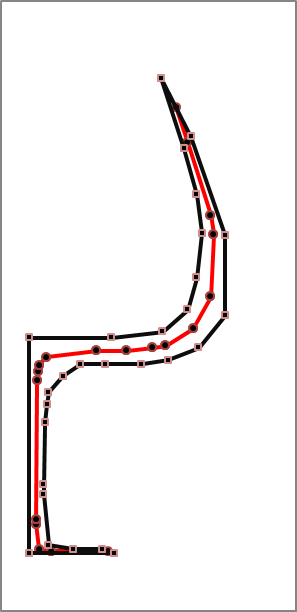
\includegraphics[angle=90,width=0.95\linewidth]{..//Common/images/Glassmc.png}} &


\raisebox{-.9\height}{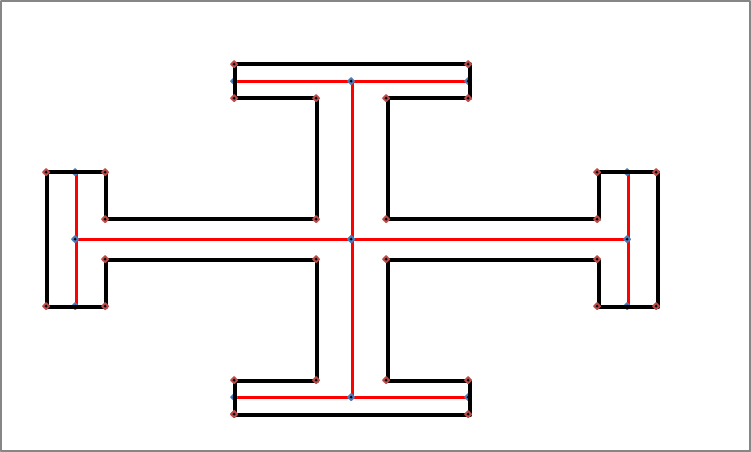
\includegraphics[width=0.85\linewidth]{..//Common/images/Crossmc.png}} \\

\end{tabular}
\end{block}

\end{column}
\end{columns}

\end{frame}
\end{document}

